Pour s'assurer de la valeur de la capacité $C$ trouvée précédemment, le
professeur réalise le montage de la
Fig.~\ref{fig:svt_national_2016_normale_phys_ex2_3} constitué des éléments
suivants~:

\begin{itemize}
    \item un générateur idéal de tension de force électromotrice $E$~;
    \item un conducteur ohmique de résistance $R=\qty{2e3}{\ohm}$~;
    \item le condensateur précédent de capacité $C$~;
    \item un interrupteur $\mathrm{K}$ à double position.
\end{itemize}

Le professeur charge totalement le condensateur en plaçant l'interrupteur en
position~(1), et puis il le bascule en position~(2) à l'instant $t_{0}=0$. Il
suit à l'aide d'un dispositif convenable les variations de la tension $u_{c}(t)$
aux bornes du condensateur.
La Fig.~\ref{fig:svt_national_2016_normale_phys_ex2_4} représente la courbe
obtenue.



\begin{minipage}{0.49\linewidth}
    \begin{figure}[H]
        \centering
        \raisebox{1cm}{%
        \begin{circuitikz}
            \newdimen\d \d=3cm
            \node[cute spdt mid,rotate=90,label=below left:$\mathrm{K}$] (s) {};
            \draw (s.out 1) node[above] {$(1)$}
                to[short] ++(-0.7\d,0)
                to[vsource,v_<=$E$] ++(0,-\d) coordinate (tmp)
                to[short] (tmp -| s.in) coordinate (tmp)
                to[C,l=$C$,v=$u_{C}$,i^<=$i$] (s.in);
            \draw (s.out 2) node[above] {$(2)$}
                to[short] ++(0.7\d,0)
                to[R,l=$R$] ++(0,-\d)
                to[short] (tmp);
        \end{circuitikz}}
        \caption{}
        \label{fig:svt_national_2016_normale_phys_ex2_3}
    \end{figure}
\end{minipage}
\hfill
\begin{minipage}{0.49\linewidth}
\begin{figure}[H]
    \centering
    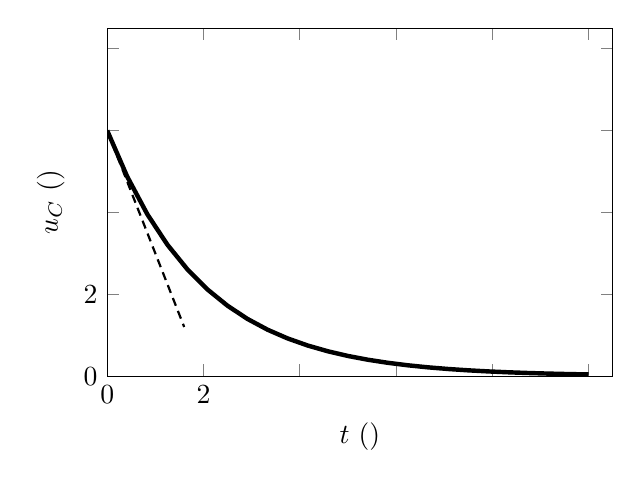
\begin{tikzpicture}[]
        \begin{axis}[
                width=8cm,height=6cm,
                xlabel=$t~(\unit{\ms})$,ylabel=$u_{C}~(\unit{\V})$,
                xmin=0,xmax=10.5,
                ymin=0,ymax=8.5,
                variable=\t,
                xtick distance=2,
                ytick distance=2,
                xticklabels={,$0$,$2$,,},
                yticklabels={,$0$,$2$,,},
            ]
            \addplot[ultra thick,domain=0:10] {6*exp(-t/2)};
            \addplot[thick,densely dashed,domain=0:1.6] {-3*t+6)};
        \end{axis}
    \end{tikzpicture}
    \caption{}
    \label{fig:svt_national_2016_normale_phys_ex2_4}
\end{figure}
\end{minipage}


\begin{enumerate}
    \item Établir l'équation différentielle vérifiée par la tension $u_{C}(t)$
          au cours de la décharge du condensateur.
    \item La solution de cette équation différentielle est de la forme
          $u_{C}(t)=A\times e^{-\frac{t}{\tau}}$. Déterminer les expressions de
          A et $\tau$ en fonction des paramètres du circuit.
    \item Déterminer graphiquement la valeur de $\tau$. Vérifier la valeur de
          $C$ trouvée dans la question~\ref{item:culcul_C}.
\end{enumerate}

